\documentclass[]{article}
\usepackage{lmodern}
\usepackage{amssymb,amsmath}
\usepackage{ifxetex,ifluatex}
\usepackage{fixltx2e} % provides \textsubscript
\ifnum 0\ifxetex 1\fi\ifluatex 1\fi=0 % if pdftex
  \usepackage[T1]{fontenc}
  \usepackage[utf8]{inputenc}
\else % if luatex or xelatex
  \ifxetex
    \usepackage{mathspec}
  \else
    \usepackage{fontspec}
  \fi
  \defaultfontfeatures{Ligatures=TeX,Scale=MatchLowercase}
\fi
% use upquote if available, for straight quotes in verbatim environments
\IfFileExists{upquote.sty}{\usepackage{upquote}}{}
% use microtype if available
\IfFileExists{microtype.sty}{%
\usepackage{microtype}
\UseMicrotypeSet[protrusion]{basicmath} % disable protrusion for tt fonts
}{}
\usepackage[margin=1in]{geometry}
\usepackage{hyperref}
\hypersetup{unicode=true,
            pdftitle={Analyzing DECREASE trials for extent of data fabrication},
            pdfauthor={Chris HJ Hartgerink, Gerben ter Riet, Marleen Kemper},
            pdfborder={0 0 0},
            breaklinks=true}
\urlstyle{same}  % don't use monospace font for urls
\usepackage{color}
\usepackage{fancyvrb}
\newcommand{\VerbBar}{|}
\newcommand{\VERB}{\Verb[commandchars=\\\{\}]}
\DefineVerbatimEnvironment{Highlighting}{Verbatim}{commandchars=\\\{\}}
% Add ',fontsize=\small' for more characters per line
\usepackage{framed}
\definecolor{shadecolor}{RGB}{248,248,248}
\newenvironment{Shaded}{\begin{snugshade}}{\end{snugshade}}
\newcommand{\KeywordTok}[1]{\textcolor[rgb]{0.13,0.29,0.53}{\textbf{{#1}}}}
\newcommand{\DataTypeTok}[1]{\textcolor[rgb]{0.13,0.29,0.53}{{#1}}}
\newcommand{\DecValTok}[1]{\textcolor[rgb]{0.00,0.00,0.81}{{#1}}}
\newcommand{\BaseNTok}[1]{\textcolor[rgb]{0.00,0.00,0.81}{{#1}}}
\newcommand{\FloatTok}[1]{\textcolor[rgb]{0.00,0.00,0.81}{{#1}}}
\newcommand{\ConstantTok}[1]{\textcolor[rgb]{0.00,0.00,0.00}{{#1}}}
\newcommand{\CharTok}[1]{\textcolor[rgb]{0.31,0.60,0.02}{{#1}}}
\newcommand{\SpecialCharTok}[1]{\textcolor[rgb]{0.00,0.00,0.00}{{#1}}}
\newcommand{\StringTok}[1]{\textcolor[rgb]{0.31,0.60,0.02}{{#1}}}
\newcommand{\VerbatimStringTok}[1]{\textcolor[rgb]{0.31,0.60,0.02}{{#1}}}
\newcommand{\SpecialStringTok}[1]{\textcolor[rgb]{0.31,0.60,0.02}{{#1}}}
\newcommand{\ImportTok}[1]{{#1}}
\newcommand{\CommentTok}[1]{\textcolor[rgb]{0.56,0.35,0.01}{\textit{{#1}}}}
\newcommand{\DocumentationTok}[1]{\textcolor[rgb]{0.56,0.35,0.01}{\textbf{\textit{{#1}}}}}
\newcommand{\AnnotationTok}[1]{\textcolor[rgb]{0.56,0.35,0.01}{\textbf{\textit{{#1}}}}}
\newcommand{\CommentVarTok}[1]{\textcolor[rgb]{0.56,0.35,0.01}{\textbf{\textit{{#1}}}}}
\newcommand{\OtherTok}[1]{\textcolor[rgb]{0.56,0.35,0.01}{{#1}}}
\newcommand{\FunctionTok}[1]{\textcolor[rgb]{0.00,0.00,0.00}{{#1}}}
\newcommand{\VariableTok}[1]{\textcolor[rgb]{0.00,0.00,0.00}{{#1}}}
\newcommand{\ControlFlowTok}[1]{\textcolor[rgb]{0.13,0.29,0.53}{\textbf{{#1}}}}
\newcommand{\OperatorTok}[1]{\textcolor[rgb]{0.81,0.36,0.00}{\textbf{{#1}}}}
\newcommand{\BuiltInTok}[1]{{#1}}
\newcommand{\ExtensionTok}[1]{{#1}}
\newcommand{\PreprocessorTok}[1]{\textcolor[rgb]{0.56,0.35,0.01}{\textit{{#1}}}}
\newcommand{\AttributeTok}[1]{\textcolor[rgb]{0.77,0.63,0.00}{{#1}}}
\newcommand{\RegionMarkerTok}[1]{{#1}}
\newcommand{\InformationTok}[1]{\textcolor[rgb]{0.56,0.35,0.01}{\textbf{\textit{{#1}}}}}
\newcommand{\WarningTok}[1]{\textcolor[rgb]{0.56,0.35,0.01}{\textbf{\textit{{#1}}}}}
\newcommand{\AlertTok}[1]{\textcolor[rgb]{0.94,0.16,0.16}{{#1}}}
\newcommand{\ErrorTok}[1]{\textcolor[rgb]{0.64,0.00,0.00}{\textbf{{#1}}}}
\newcommand{\NormalTok}[1]{{#1}}
\usepackage{longtable,booktabs}
\usepackage{graphicx,grffile}
\makeatletter
\def\maxwidth{\ifdim\Gin@nat@width>\linewidth\linewidth\else\Gin@nat@width\fi}
\def\maxheight{\ifdim\Gin@nat@height>\textheight\textheight\else\Gin@nat@height\fi}
\makeatother
% Scale images if necessary, so that they will not overflow the page
% margins by default, and it is still possible to overwrite the defaults
% using explicit options in \includegraphics[width, height, ...]{}
\setkeys{Gin}{width=\maxwidth,height=\maxheight,keepaspectratio}
\IfFileExists{parskip.sty}{%
\usepackage{parskip}
}{% else
\setlength{\parindent}{0pt}
\setlength{\parskip}{6pt plus 2pt minus 1pt}
}
\setlength{\emergencystretch}{3em}  % prevent overfull lines
\providecommand{\tightlist}{%
  \setlength{\itemsep}{0pt}\setlength{\parskip}{0pt}}
\setcounter{secnumdepth}{0}
% Redefines (sub)paragraphs to behave more like sections
\ifx\paragraph\undefined\else
\let\oldparagraph\paragraph
\renewcommand{\paragraph}[1]{\oldparagraph{#1}\mbox{}}
\fi
\ifx\subparagraph\undefined\else
\let\oldsubparagraph\subparagraph
\renewcommand{\subparagraph}[1]{\oldsubparagraph{#1}\mbox{}}
\fi

%%% Use protect on footnotes to avoid problems with footnotes in titles
\let\rmarkdownfootnote\footnote%
\def\footnote{\protect\rmarkdownfootnote}

%%% Change title format to be more compact
\usepackage{titling}

% Create subtitle command for use in maketitle
\newcommand{\subtitle}[1]{
  \posttitle{
    \begin{center}\large#1\end{center}
    }
}

\setlength{\droptitle}{-2em}
  \title{Analyzing DECREASE trials for extent of data fabrication}
  \pretitle{\vspace{\droptitle}\centering\huge}
  \posttitle{\par}
  \author{Chris HJ Hartgerink, Gerben ter Riet, Marleen Kemper}
  \preauthor{\centering\large\emph}
  \postauthor{\par}
  \predate{\centering\large\emph}
  \postdate{\par}
  \date{26 January, 2017}


\begin{document}
\maketitle

The effect of beta-blockers on perioperative mortality in non-cardiac
surgery for patients with coronary artery disease (CAD) has been subject
of discussion\textsuperscript{1} due to findings of research
misconduct\textsuperscript{2--4} that were central to claims of their
effectiveness\textsuperscript{5--7}. Perioperative mortality is the
deathrate of patients during the period of the surgical procedure, which
typically includes admission, anaesthesia, surgery, and recovery. This
related finding of research misconduct altered meta-analytic results of
perioperative mortality in non-cardiac surgery for CAD patients
substantively\textsuperscript{7}, where meta-analyses that include these
studies conclude that beta-blockers decrease perioperative
mortality\textsuperscript{5--7} but a meta-analysis that excludes these
studies concludes that beta-blockers increase perioperative
mortality\textsuperscript{7}.

The trials deemed to be the result of research misconduct were the Dutch
DECREASE trials\textsuperscript{2--4}. The committees that investigated
the integrity of the DECREASE studies reported that data fabrication was
likely\textsuperscript{2--4}, but that the extent of the data
fabrication remained unclear. Given that the inclusion or exclusion of
these trials in meta-analyses is crucial in determining whether
beta-blockers are indeed effective during the perioperative period and
the latest guidelines still recommend the usage of
beta-blockers\textsuperscript{8}, we aim to estimate the extent of data
fabrication in the DECREASE studies\textsuperscript{9,10} in order to
further this debate.

The reports on the DECREASE trials primarily focused on the provenance
of the raw data and patient files (e.g., informed consent, whether data
corresponded to patient files), but neglected the extent to which the
DECREASE studies deviated from similar trials that tested the
effectiveness of beta-blockers on perioperative mortality. Comparing how
(dis)similar trials are from comparable studies is not a new
idea\textsuperscript{11} and has proven effective in detecting data
fabrication\textsuperscript{12}. This is a different approach from the
forensic statistical methods previously applied\textsuperscript{4},
where results within one study are evaluated as opposed to other similar
studies. This explains the discrepancy between the feasibility of
evaluating the DECREASE trials by the statistical expert of the
committee report and ours.

To statistically investigate the evidence of data fabrication in the
results of the DECREASE studies\textsuperscript{9,10}, we took three
steps. First, we replicate the findings from a 2014
meta-analysis\textsuperscript{7} that contains sufficient information to
estimate the deviation of the DECREASE-I and DECREASE-IV studies from
the remaining studies. Second, we evaluate the veracity of the
DECREASE-I and DECREASE-IV studies (i.e., the probability that these
study findings occurred assuming no data fabrication occurred). Third,
we reverse this assumption and assume that data fabrication did occur
and estimate how many data points would have to be fabricated to
reproduce the results of the DECREASE-I and DECREASE-IV studies if the
remaining studies are regarded as estimating the true effect of
beta-blockers on perioperative mortality.

\section{Step 1: reproducing meta-analysis of Bouri et al.
(2014)}\label{step-1-reproducing-meta-analysis-of-bouri-et-al.-2014}

\subsection{Methods}\label{methods}

To ensure that we used similar analysis procedures as in the 2014
meta-analysis\textsuperscript{7}, we initially reproduced Bouri et al.'s
estimates. This ensured that (1) their results are reproducible and (2)
we are using the correct estimates in subsequent steps of our analyses.
Using figures 2 and 3 from the original paper\textsuperscript{7}, we
extracted the raw event data for the 2 (control vs experimental) by 2
(event or no event) design, which we used to recompute the natural
logarithm of the risk ratio and its standard error. The extracted event
data is available at \href{https://osf.io/aykeh}{osf.io/aykeh} and our
analysis plan was preregistered at
\href{https://osf.io/vnmzc}{osf.io/vnmzc}.

We computed the log risk ratio (i.e., log RR) for each study and pooled
these using the \texttt{R} package \texttt{metafor}\textsuperscript{13}.
We estimated a weighted random-effects model using the restricted
maximum-likelihood estimator (i.e., \texttt{REML})\textsuperscript{14}
to estimate the variance of effects. We used the default weighting
procedure in the \texttt{metafor} package. When there was a zero-count
for a cell, .5 was added to each cell of that trial, as is common in
meta-analyses on risk- and odds ratios in order to deal with
computational artefacts\textsuperscript{15}. The 2014
meta-analysis\textsuperscript{7} did not specify the effect variance
estimate used; hence, minor discrepancies between our estimates and the
original estimates could be due to differences in the estimation
procedure.

\subsection{Results}\label{results}

We analyzed the RRs to verify the original estimates (Figure 2 of the
2014 meta-analysis\textsuperscript{7}) and found that we were able to
reproduce the estimates for the different sets of studies. Bouri et al.
differentiated between the estimates from the non-DECREASE trials and
the DECREASE trials. We confirmed the effect size estimates and the
variance estimates for both the non-DECREASE- and the DECREASE trials,
save for some minor discrepancies due to the estimation method. Table 1
depicts the original and reproduced values for both sets of studies.

\begin{longtable}[]{@{}lllll@{}}
\caption{The original- and reproduced meta-analytic results based on the
data provided in the 2014 meta-analysis by Bouri et al.}\tabularnewline
\toprule
& & Risk ratio & \(\tau^2\) & Confidence interval\tabularnewline
Non-DECREASE & Original & 1.27 & 0 & {[}1.01; 1.60{]}\tabularnewline
& Reproduced & 1.28 & 0 & {[}1.01; 1.62{]}\tabularnewline
DECREASE & Original & 0.42 & 0.29 & {[}0.15; 1.23{]}\tabularnewline
& Reproduced & 0.44 & 0.24 & {[}0.15; 1.23{]}\tabularnewline
\bottomrule
\end{longtable}

Second, we meta-analyzed all studies combined, including a dummy
predictor for the DECREASE and non-DECREASE studies to replicate results
presented in Figure 4 of the 2014 meta-analysis\textsuperscript{7}.
Surprisingly, our results showed more evidence for unequal subgroups
than the original meta-analysis\textsuperscript{7}; whereas the original
test for subgroup differences was \(\chi^2(1)=3.91,p=.05\), our analyses
indicated that \(\chi^2(1)=6.12,p=0.013\). Additionally, the original
analyses showed substantial heterogeneity (\(I^2=74.4\)\%) where we
found an \(I^2=0\)\%. Different heterogeneity estimators (e.g.,
\texttt{DerSimonian-Laird} instead of \texttt{REML}) did not resolve
this difference. We tried to clarify these discrepancies by e-mailing
the original authors, but failed to receive a response.

\section{Step 2: evaluating the veracity of DECREASE
studies}\label{step-2-evaluating-the-veracity-of-decrease-studies}

Based on the non-DECREASE estimates from Step 1, we estimated the
probability of obtaining the results in the DECREASE studies. To this
end, we assumed that the non-DECREASE studies provide a valid
representation of the true effect of beta-blockers on perioperative
mortality (similar to Bouri et al.\textsuperscript{7}; but see the
discussion). The estimated probability is also known as the veracity of
the data\textsuperscript{16}, which indicates the probability of the
observed data under a given true effect. We assumed that the
non-DECREASE studies estimate the true population distribution of
effects, not perturbed by publication bias due to statistical
(non)significance. Publication bias was assumed to not be a problem
because a substantial number of nonsignificant effects are included in
the dataset (9 of 11 nonsignificant).

\subsection{Method}\label{method}

Based on the estimated mean log RR and its credible interval in the
non-DECREASE studies, we computed the probability of log RR in the
DECREASE trials. The estimates of the non-DECREASE studies were obtained
from Step 1, which include the estimated log RR (i.e., 0.25), and its
95\% credibility interval as provided by the package \texttt{metafor}
(i.e., {[}0.01; 0.484{]}. We assumed a normal distribution of population
effects with the estimated effect as the mean of the distribution. The
95\% credibility interval denotes the bounds of the normal distribution
that covers 95\% of the density, where the standard deviation is
calculated as the distance from the mean to either bound, divided by
1.96. This allows for an approximation of the population effect
distribution, as depicted in Figure 1.

\begin{figure}

{\centering 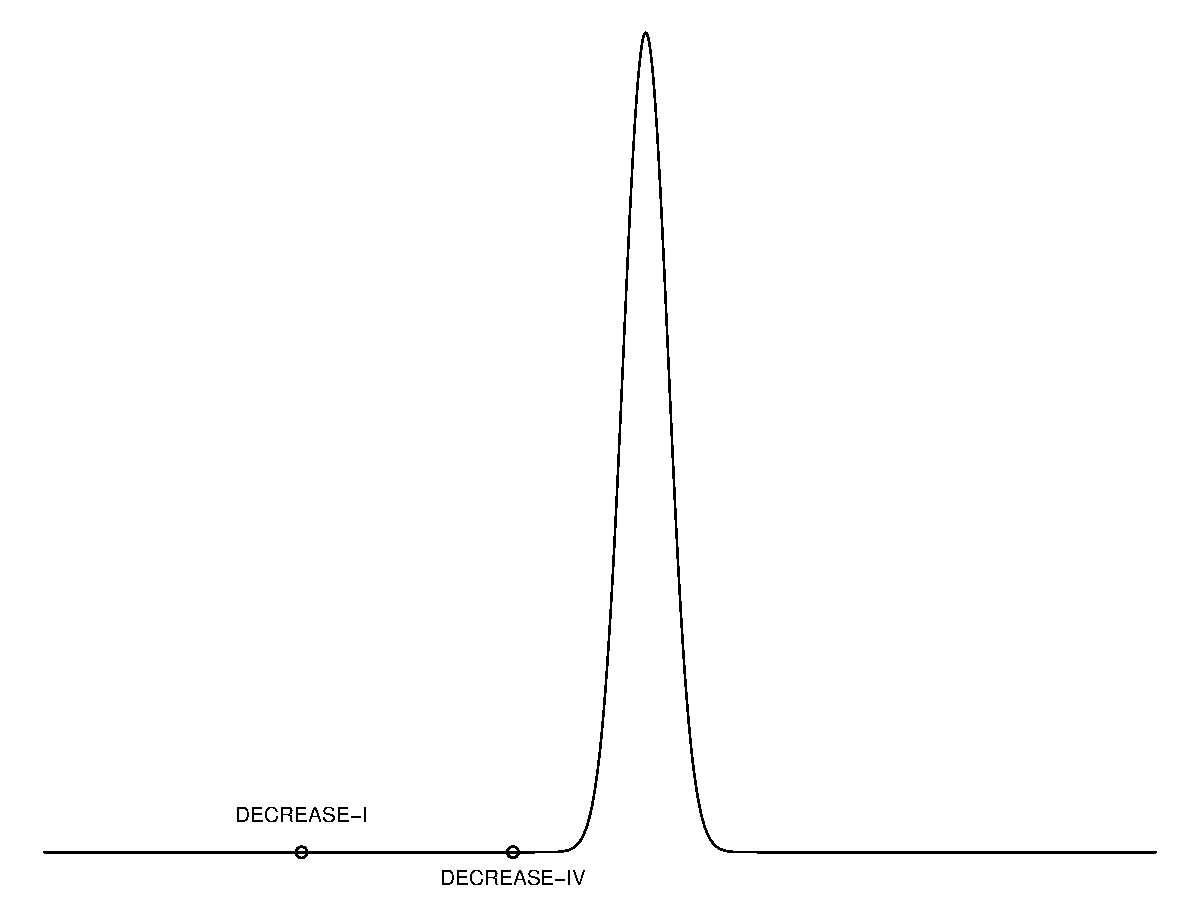
\includegraphics[width=0.8\linewidth]{../figures/fig1} 

}

\caption{Density plot of the estimated true effect distribution based on the non-DECREASE studies only, with the position of the DECREASE studies highlighted.}\label{fig:figure 1}
\end{figure}

Based on the estimated effect distribution from the non-DECREASE trials,
we calculated the probability of each DECREASE trial result, or a more
extreme result. In other words, we computed the \emph{p}-value for the
hypothesis that the DECREASE studies occurred based on the information
available from the other trials.

\subsection{Results}\label{results-1}

Figure 1 indicates that the DECREASE trials are highly unlikely under
the estimated effect distribution based on the non-DECREASE trials. More
specifically, DECREASE-I (or more extreme) has a probability of
\(2.9610213\times 10^{-53}\) (less than 1 in a quintillion) and
DECREASE-IV \(3.0974376\times 10^{-9}\) (3 in a billion), which
indicates they are unlikely to come from the same population effect
distribution as the non-DECREASE trials. Observing two of such extremely
unlikely results in this population effect distribution jointly is
highly improbable, \(9.1715786\times 10^{-62}\). This would therefore
indicate that the DECREASE trials are severely different from the
non-DECREASE studies.

Results from Step 1 indicated that no variance (i.e., homogeneity;
\(\tau^2=0\)) of the effects was observed; given the small number of
studies included (i.e., 9) this estimate is uncertain, however. We
conducted sensitivity analyses in order to see how dependent results are
on the specific heterogeneity estimate. The probability of observing
both DECREASE trials stays approximately below 1 out of 1000 until the
variance estimate is .25, and the probability stays approximately below
1 out of 100 until the variance estimate is .43 (see Figure 2). Further
research would be worthwhile to better estimate the variance in the
effects of beta-blockers on perioperative mortality and what moderators
affect the effect size (e.g., type of beta-blocker).

\begin{figure}

{\centering 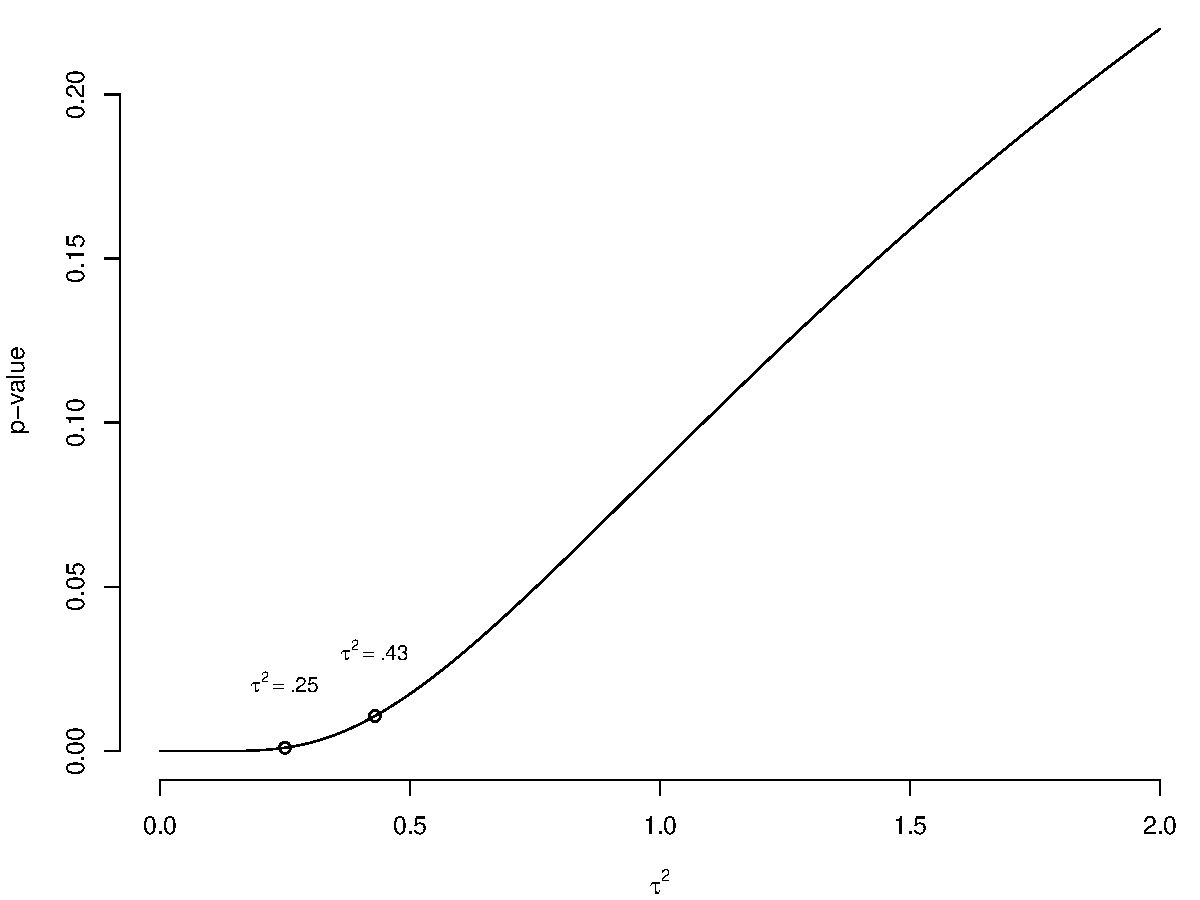
\includegraphics[width=0.8\linewidth]{../figures/fig2} 

}

\caption{Sensitivity analyses for the p-value that indicates the probability of observing the results from the DECREASE studies, or more extreme results, based on the estimated true effect (non-DECREASE trials) and the accompanying variance estimate.}\label{fig:figure 2}
\end{figure}

\section{Step 3: estimating the amount of fabricated
data}\label{step-3-estimating-the-amount-of-fabricated-data}

We estimated the number of data points that would need to be fabricated
to arrive at the estimates from the DECREASE studies, given that the
non-DECREASE studies represent the true effect. This assumes, in
contrast to Step 2, that the DECREASE studies in fact contain fabricated
data. The estimates from Step 3 provide an indication of the extent of
the potential data fabrication in the DECREASE studies under this
assumption\textsuperscript{2--4,7}.

\subsection{Method}\label{method-1}

In order to estimate the number of fabricated data points, we estimated
the population effect distribution of mortality (in log odds) per
condition in both the DECREASE- and non-DECREASE studies separately. For
each of these, we ran a meta-analysis applying the same, verified
methods used in Step 1. These separate analyses were necessary,
considering that Step 1 only provided estimates of the overall risk
ratio but not the odds conditional on exposure (beta-blocker or control)
and study set (DECREASE- versus non-DECREASE). This resulted in four
meta-analytic mortality estimates with an accompanying variance.
Throughout the simulations, we use the point estimates to simulate
genuine- and fabricated data, but supplement this by using the
distribution estimates as sensitivity analyses.

We applied the inversion method to estimate the number of fabricated
data points in the DECREASE-I and DECREASE-IV
studies\textsuperscript{17}. With the inversion method, we iteratively
hypothesized that \emph{X} out of \emph{N} data points were fabricated
(i.e., \(0, 1, ..., N\)) in the DECREASE-I and DECREASE-IV studies
separately. For each study, we simulated 10,000 datasets per hypothesis
of \emph{X} fabricated data points and \emph{N-X} genuine data points.
For each simulated dataset (exact simulation procedure in next
paragraph), we determined the likelihood of the results with

\begin{equation}
\label{eq1}
L(\theta|\pi_{E},\pi_{C})=\pi_{E}^{n_{11}}(1-\pi_{E})^{n_{12}} \times \pi_{C}^{n_{21}}(1 - \pi_{C})^{n_{22}}
\end{equation}

where \(\pi_{E}\) indicates the mortality rate of the experimental
condition as drawn from the meta-analytic effect distribution
(\(\pi_{C}\) indicates the same for the control condition). The
likelihood was computed under both the fabricated effect estimates
(i.e., \(L_{fabricated}\)) and the genuine data (i.e., \(L_{genuine}\)).
Table 2 indicates which cell sizes the various \(n_{XX}\) refer to
within the (simulated) data. We compared the likelihoods to determine
whether the simulated data were more likely to arise from the genuine-
(\(L_{genuine}\)) or from the fabricated data (\(L_{fabricated}\)). Note
that using the likelihoods for this is a minor deviation from the
preregistration, where we initially planned on using \(p\)-value
comparisons (\href{https://osf.io/vnmzc}{osf.io/vnmzc}).

\begin{longtable}[]{@{}lll@{}}
\caption{Outcome possibilities within a simulated 2 (beta-blocker v
control) by 2 (dead v alive) clinical trial.}\tabularnewline
\toprule
& Dead & Alive\tabularnewline
Beta-blockers & \(n_{11}\) & \(n_{12}\)\tabularnewline
Control & \(n_{21}\) & \(n_{22}\)\tabularnewline
\bottomrule
\end{longtable}

For each hypothesis of \emph{X} out of \emph{N} fabricated datapoints,
we computed the probability that the fabricated data are more likely
than the genuine data (\(p_F=P(L_{fabricated}>L_{genuine})\)). Based on
\(p_F\), we computed the confidence interval for \(X\) (i.e.,
\(X_{LB};X_{UB}\)). For a 95\% confidence interval, the lowerbound is
equal to the \(p_F\) closest to .025, whereas the upperbound is equal to
the \(p_F\) closest to .975.

We computed \(p_F\) for all possibilities of \emph{X} out of \emph{N}
fabricated datapoints in 10,000 randomly generated datsets, which were
generated in three steps. For each dataset we:

\begin{enumerate}
\def\labelenumi{\arabic{enumi}.}
\item
  Sampled (without replacement) \emph{X} fictitious participants that
  would be the result of data fabrication (sampled across all
  conditions).
\item
  Determined the population mortality rate for each condition (i.e., for
  each cell as in Table 3). The meta-analytic point estimate was used or
  a population effect was randomly drawn from the meta-analytic effect
  distribution.
\item
  Simulated the number of deaths for the different conditions using a
  binomial distribution based on the mortality rate as determined in 2,
  resulting in the cell counts as in Table 3.
\end{enumerate}

Based on the meta-analytic effect from 2 and the cell sizes from 3, we
computed the likelihoods of \(L_{fabricated}\) and \(L_{genuine}\) using
Equation \ref{eq1}. As mentioned before, \(p_F\) was computed as the
probability that the data were more likely under the estimates resulting
from the (allegedly) fabricated data (i.e., the DECREASE trials) than
under the estimates resulting from the genuine data (i.e., the
non-DECREASE trials; \(p_F=P(L_{fabricated}>L_{genuine})\)).

\subsection{Results}\label{results-2}

\begin{figure}

{\centering 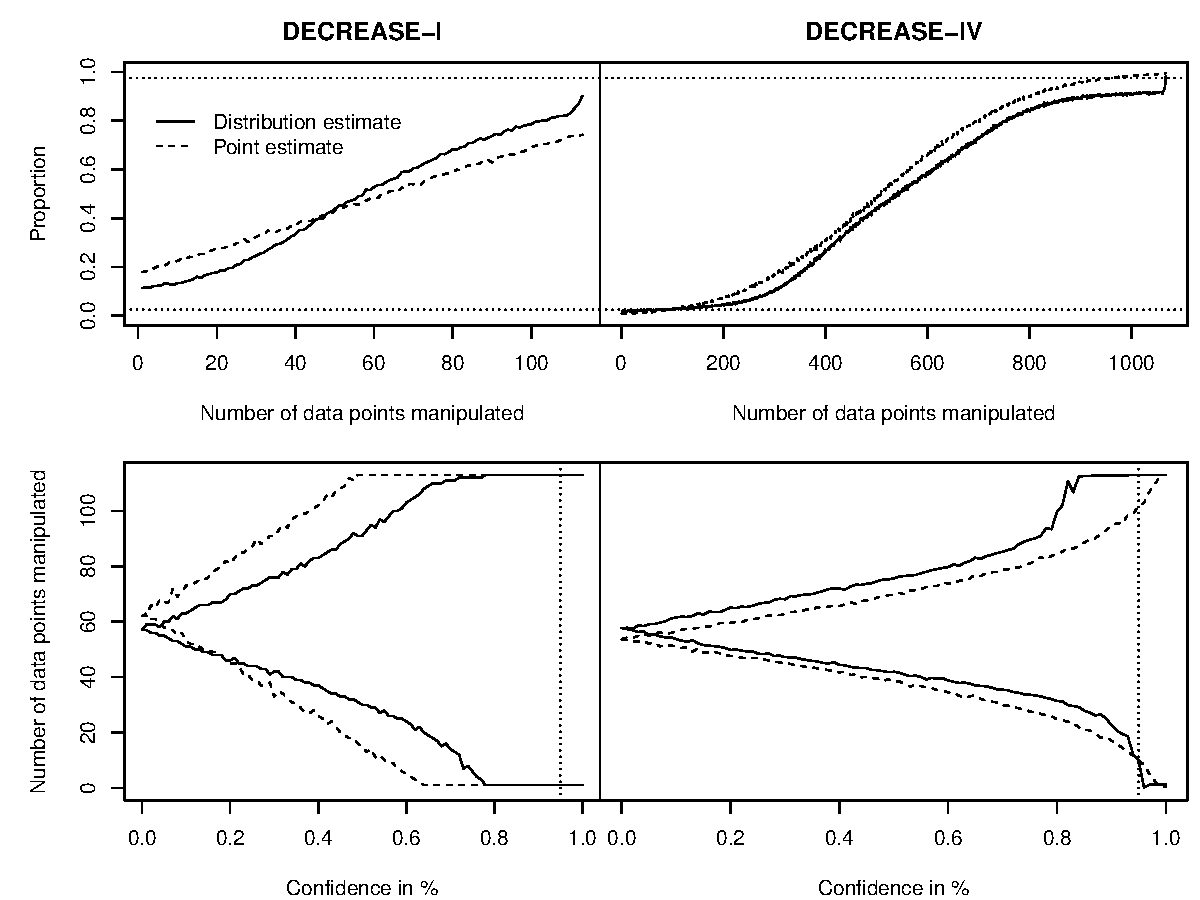
\includegraphics[width=0.8\linewidth]{../figures/fig3} 

}

\caption{Test}\label{fig:figure 3}
\end{figure}

\begin{Shaded}
\begin{Highlighting}[]
\NormalTok{res_i_certain}
\end{Highlighting}
\end{Shaded}

\begin{verbatim}
##   [1] 0.1507 0.1624 0.1700 0.1674 0.1792 0.1807 0.1868 0.1867 0.1879 0.1930
##  [11] 0.2012 0.2182 0.2083 0.2114 0.2257 0.2296 0.2361 0.2476 0.2377 0.2488
##  [21] 0.2545 0.2631 0.2742 0.2788 0.2823 0.2894 0.3002 0.2996 0.3032 0.3094
##  [31] 0.3180 0.3243 0.3305 0.3352 0.3380 0.3547 0.3575 0.3649 0.3740 0.3873
##  [41] 0.3852 0.3957 0.4099 0.4088 0.4113 0.4205 0.4314 0.4378 0.4430 0.4524
##  [51] 0.4643 0.4655 0.4651 0.4851 0.4983 0.4931 0.5006 0.5106 0.5148 0.5241
##  [61] 0.5338 0.5428 0.5528 0.5549 0.5558 0.5768 0.5752 0.5797 0.5912 0.6043
##  [71] 0.6060 0.6177 0.6243 0.6283 0.6346 0.6433 0.6515 0.6586 0.6667 0.6684
##  [81] 0.6787 0.6895 0.6947 0.6978 0.7021 0.7121 0.7150 0.7264 0.7287 0.7402
##  [91] 0.7401 0.7522 0.7506 0.7533 0.7591 0.7762 0.7832 0.7782 0.7821 0.7873
## [101] 0.7894 0.7925 0.8009 0.8095 0.8175 0.8135 0.8211 0.8251 0.8306 0.8363
## [111] 0.8349 0.8372 0.8453
\end{verbatim}

\begin{Shaded}
\begin{Highlighting}[]
\NormalTok{res_i_uncertain}
\end{Highlighting}
\end{Shaded}

\begin{verbatim}
##   [1] 0.1224 0.1247 0.1263 0.1213 0.1224 0.1318 0.1288 0.1355 0.1370 0.1419
##  [11] 0.1502 0.1448 0.1557 0.1582 0.1619 0.1730 0.1801 0.1758 0.1796 0.1869
##  [21] 0.1938 0.1968 0.2086 0.2106 0.2239 0.2267 0.2350 0.2414 0.2446 0.2602
##  [31] 0.2619 0.2716 0.2697 0.2896 0.3045 0.3067 0.3302 0.3313 0.3332 0.3543
##  [41] 0.3552 0.3801 0.3755 0.3816 0.4068 0.4056 0.4106 0.4231 0.4297 0.4384
##  [51] 0.4573 0.4694 0.4742 0.4911 0.4864 0.5000 0.5125 0.5172 0.5247 0.5337
##  [61] 0.5451 0.5518 0.5554 0.5640 0.5666 0.5798 0.5924 0.5896 0.6015 0.6100
##  [71] 0.6154 0.6297 0.6251 0.6376 0.6446 0.6480 0.6616 0.6649 0.6725 0.6786
##  [81] 0.6887 0.6913 0.6999 0.7077 0.7116 0.7248 0.7153 0.7227 0.7302 0.7379
##  [91] 0.7432 0.7499 0.7534 0.7530 0.7567 0.7708 0.7712 0.7762 0.7723 0.7988
## [101] 0.7908 0.7958 0.7998 0.8060 0.8082 0.8051 0.8234 0.8162 0.8240 0.8323
## [111] 0.8445 0.8647 0.8862
\end{verbatim}

\begin{Shaded}
\begin{Highlighting}[]
\NormalTok{res_iv_certain}
\end{Highlighting}
\end{Shaded}

\begin{verbatim}
##    [1] 0.0223 0.0255 0.0234 0.0240 0.0263 0.0263 0.0226 0.0232 0.0220
##   [10] 0.0234 0.0251 0.0254 0.0247 0.0234 0.0276 0.0249 0.0268 0.0244
##   [19] 0.0244 0.0275 0.0264 0.0267 0.0267 0.0250 0.0279 0.0253 0.0254
##   [28] 0.0268 0.0267 0.0267 0.0267 0.0257 0.0264 0.0279 0.0264 0.0274
##   [37] 0.0285 0.0295 0.0269 0.0290 0.0301 0.0305 0.0288 0.0281 0.0271
##   [46] 0.0293 0.0280 0.0271 0.0266 0.0289 0.0283 0.0277 0.0299 0.0283
##   [55] 0.0296 0.0326 0.0344 0.0291 0.0321 0.0299 0.0287 0.0302 0.0289
##   [64] 0.0301 0.0297 0.0312 0.0315 0.0291 0.0308 0.0300 0.0298 0.0319
##   [73] 0.0283 0.0339 0.0311 0.0317 0.0313 0.0322 0.0324 0.0342 0.0302
##   [82] 0.0334 0.0332 0.0340 0.0334 0.0328 0.0349 0.0334 0.0348 0.0339
##   [91] 0.0339 0.0326 0.0350 0.0324 0.0353 0.0307 0.0339 0.0386 0.0379
##  [100] 0.0343 0.0347 0.0356 0.0370 0.0358 0.0343 0.0345 0.0356 0.0373
##  [109] 0.0399 0.0382 0.0376 0.0372 0.0376 0.0383 0.0374 0.0391 0.0349
##  [118] 0.0389 0.0377 0.0406 0.0443 0.0394 0.0402 0.0415 0.0406 0.0415
##  [127] 0.0412 0.0433 0.0430 0.0376 0.0399 0.0444 0.0418 0.0445 0.0464
##  [136] 0.0450 0.0461 0.0421 0.0447 0.0398 0.0418 0.0440 0.0461 0.0463
##  [145] 0.0500 0.0447 0.0438 0.0439 0.0492 0.0465 0.0464 0.0466 0.0487
##  [154] 0.0482 0.0467 0.0530 0.0501 0.0466 0.0510 0.0470 0.0540 0.0517
##  [163] 0.0542 0.0523 0.0549 0.0488 0.0509 0.0550 0.0550 0.0525 0.0541
##  [172] 0.0522 0.0579 0.0551 0.0548 0.0533 0.0590 0.0573 0.0557 0.0572
##  [181] 0.0548 0.0531 0.0598 0.0566 0.0613 0.0595 0.0599 0.0545 0.0627
##  [190] 0.0581 0.0625 0.0603 0.0643 0.0595 0.0650 0.0621 0.0657 0.0673
##  [199] 0.0648 0.0666 0.0684 0.0676 0.0654 0.0673 0.0679 0.0702 0.0687
##  [208] 0.0749 0.0713 0.0731 0.0696 0.0709 0.0702 0.0719 0.0764 0.0758
##  [217] 0.0733 0.0790 0.0725 0.0773 0.0770 0.0765 0.0778 0.0822 0.0789
##  [226] 0.0801 0.0814 0.0858 0.0820 0.0821 0.0854 0.0803 0.0824 0.0831
##  [235] 0.0864 0.0895 0.0845 0.0943 0.0883 0.0963 0.0930 0.0919 0.0871
##  [244] 0.0921 0.0940 0.0896 0.0967 0.0941 0.1000 0.0969 0.0980 0.0951
##  [253] 0.0988 0.1051 0.1031 0.1013 0.1059 0.0974 0.1055 0.1064 0.1074
##  [262] 0.1058 0.1068 0.1064 0.1117 0.1100 0.1069 0.1174 0.1078 0.1120
##  [271] 0.1107 0.1124 0.1180 0.1165 0.1190 0.1238 0.1187 0.1207 0.1219
##  [280] 0.1310 0.1247 0.1233 0.1288 0.1228 0.1319 0.1248 0.1337 0.1326
##  [289] 0.1339 0.1346 0.1329 0.1365 0.1366 0.1443 0.1395 0.1391 0.1377
##  [298] 0.1433 0.1424 0.1435 0.1466 0.1503 0.1519 0.1494 0.1459 0.1519
##  [307] 0.1578 0.1559 0.1500 0.1585 0.1550 0.1520 0.1651 0.1632 0.1662
##  [316] 0.1605 0.1623 0.1672 0.1663 0.1654 0.1730 0.1665 0.1721 0.1663
##  [325] 0.1789 0.1690 0.1754 0.1792 0.1782 0.1825 0.1827 0.1846 0.1820
##  [334] 0.1861 0.1884 0.1893 0.1936 0.1931 0.1956 0.1903 0.1942 0.1914
##  [343] 0.1901 0.2079 0.2054 0.2033 0.1976 0.2029 0.2099 0.2079 0.2084
##  [352] 0.2212 0.2063 0.2079 0.2232 0.2101 0.2222 0.2166 0.2184 0.2144
##  [361] 0.2220 0.2219 0.2351 0.2272 0.2271 0.2311 0.2337 0.2291 0.2382
##  [370] 0.2409 0.2362 0.2391 0.2327 0.2468 0.2372 0.2416 0.2520 0.2460
##  [379] 0.2548 0.2598 0.2457 0.2585 0.2620 0.2636 0.2608 0.2623 0.2661
##  [388] 0.2669 0.2655 0.2664 0.2662 0.2679 0.2702 0.2770 0.2752 0.2769
##  [397] 0.2836 0.2842 0.2828 0.2806 0.2860 0.2825 0.2788 0.2874 0.2987
##  [406] 0.2879 0.2975 0.2895 0.2920 0.3043 0.3040 0.3044 0.3065 0.3083
##  [415] 0.3066 0.3182 0.3098 0.3150 0.3167 0.3066 0.3137 0.3200 0.3153
##  [424] 0.3271 0.3237 0.3273 0.3252 0.3359 0.3381 0.3298 0.3320 0.3384
##  [433] 0.3328 0.3353 0.3417 0.3377 0.3521 0.3491 0.3432 0.3503 0.3540
##  [442] 0.3581 0.3569 0.3499 0.3632 0.3561 0.3652 0.3658 0.3703 0.3630
##  [451] 0.3637 0.3745 0.3743 0.3858 0.3751 0.3728 0.3801 0.3978 0.3775
##  [460] 0.3776 0.3882 0.3847 0.3893 0.3876 0.3899 0.3889 0.3906 0.3921
##  [469] 0.4023 0.4096 0.4099 0.4129 0.4029 0.4086 0.4096 0.4102 0.4108
##  [478] 0.4269 0.4119 0.4128 0.4277 0.4196 0.4194 0.4236 0.4307 0.4253
##  [487] 0.4279 0.4335 0.4413 0.4325 0.4449 0.4420 0.4371 0.4446 0.4488
##  [496] 0.4494 0.4533 0.4548 0.4574 0.4723 0.4585 0.4768 0.4649 0.4670
##  [505] 0.4617 0.4672 0.4727 0.4755 0.4753 0.4681 0.4862 0.4814 0.4835
##  [514] 0.4873 0.4832 0.4794 0.4749 0.4809 0.4973 0.4886 0.4986 0.4971
##  [523] 0.5020 0.4994 0.5077 0.5026 0.5016 0.5028 0.5094 0.5111 0.5157
##  [532] 0.5163 0.5252 0.5159 0.5145 0.5301 0.5237 0.5264 0.5364 0.5265
##  [541] 0.5337 0.5342 0.5420 0.5380 0.5473 0.5335 0.5496 0.5520 0.5463
##  [550] 0.5514 0.5471 0.5465 0.5572 0.5573 0.5569 0.5582 0.5618 0.5581
##  [559] 0.5711 0.5598 0.5705 0.5692 0.5758 0.5841 0.5741 0.5778 0.5785
##  [568] 0.5856 0.5898 0.5809 0.5956 0.5882 0.5916 0.6016 0.5906 0.5955
##  [577] 0.6025 0.6019 0.5995 0.5995 0.6165 0.6099 0.6058 0.6030 0.6195
##  [586] 0.6180 0.6142 0.6274 0.6210 0.6202 0.6308 0.6285 0.6253 0.6296
##  [595] 0.6348 0.6360 0.6446 0.6328 0.6408 0.6404 0.6390 0.6490 0.6529
##  [604] 0.6408 0.6524 0.6547 0.6440 0.6573 0.6582 0.6538 0.6579 0.6646
##  [613] 0.6699 0.6688 0.6707 0.6745 0.6714 0.6767 0.6739 0.6773 0.6863
##  [622] 0.6772 0.6827 0.6887 0.6903 0.6890 0.6941 0.7070 0.6965 0.6978
##  [631] 0.7017 0.7021 0.7107 0.6981 0.7082 0.7076 0.7137 0.7035 0.7197
##  [640] 0.7202 0.7168 0.7055 0.7230 0.7291 0.7289 0.7301 0.7281 0.7277
##  [649] 0.7348 0.7312 0.7336 0.7395 0.7424 0.7412 0.7415 0.7463 0.7491
##  [658] 0.7462 0.7457 0.7517 0.7573 0.7553 0.7580 0.7545 0.7525 0.7570
##  [667] 0.7567 0.7598 0.7663 0.7682 0.7717 0.7640 0.7707 0.7705 0.7758
##  [676] 0.7772 0.7756 0.7817 0.7779 0.7849 0.7966 0.7825 0.7862 0.7937
##  [685] 0.7902 0.7972 0.7933 0.7858 0.7964 0.7949 0.7984 0.8011 0.7970
##  [694] 0.8021 0.8076 0.8037 0.8106 0.8091 0.8119 0.8136 0.8124 0.8093
##  [703] 0.8086 0.8218 0.8195 0.8156 0.8202 0.8175 0.8287 0.8196 0.8284
##  [712] 0.8299 0.8276 0.8316 0.8237 0.8336 0.8291 0.8418 0.8362 0.8353
##  [721] 0.8376 0.8431 0.8465 0.8381 0.8416 0.8450 0.8416 0.8426 0.8440
##  [730] 0.8507 0.8440 0.8547 0.8493 0.8567 0.8528 0.8445 0.8588 0.8619
##  [739] 0.8548 0.8633 0.8534 0.8626 0.8626 0.8691 0.8658 0.8619 0.8686
##  [748] 0.8607 0.8693 0.8702 0.8726 0.8731 0.8749 0.8682 0.8763 0.8730
##  [757] 0.8717 0.8712 0.8751 0.8813 0.8830 0.8812 0.8811 0.8749 0.8830
##  [766] 0.8878 0.8838 0.8891 0.8871 0.8890 0.8866 0.8868 0.8898 0.8901
##  [775] 0.8863 0.8902 0.8962 0.8903 0.8947 0.8978 0.8944 0.8937 0.8985
##  [784] 0.9033 0.8936 0.8980 0.8984 0.9069 0.9011 0.8996 0.8956 0.9031
##  [793] 0.9007 0.8993 0.9015 0.9057 0.9060 0.9110 0.9130 0.9038 0.9040
##  [802] 0.9148 0.9115 0.9110 0.9132 0.9139 0.9179 0.9140 0.9089 0.9152
##  [811] 0.9162 0.9185 0.9105 0.9173 0.9160 0.9187 0.9176 0.9189 0.9184
##  [820] 0.9203 0.9191 0.9229 0.9214 0.9153 0.9251 0.9215 0.9259 0.9267
##  [829] 0.9177 0.9222 0.9312 0.9247 0.9366 0.9263 0.9303 0.9284 0.9276
##  [838] 0.9307 0.9288 0.9293 0.9293 0.9359 0.9324 0.9297 0.9346 0.9323
##  [847] 0.9352 0.9317 0.9365 0.9337 0.9354 0.9308 0.9316 0.9351 0.9386
##  [856] 0.9377 0.9344 0.9406 0.9388 0.9386 0.9362 0.9395 0.9396 0.9396
##  [865] 0.9381 0.9383 0.9376 0.9385 0.9422 0.9423 0.9404 0.9430 0.9417
##  [874] 0.9422 0.9380 0.9408 0.9443 0.9423 0.9462 0.9469 0.9467 0.9440
##  [883] 0.9466 0.9462 0.9533 0.9399 0.9487 0.9491 0.9492 0.9480 0.9446
##  [892] 0.9450 0.9462 0.9528 0.9501 0.9479 0.9495 0.9484 0.9501 0.9504
##  [901] 0.9486 0.9540 0.9497 0.9506 0.9538 0.9524 0.9517 0.9547 0.9528
##  [910] 0.9522 0.9551 0.9545 0.9558 0.9550 0.9537 0.9496 0.9515 0.9547
##  [919] 0.9542 0.9546 0.9520 0.9533 0.9557 0.9555 0.9530 0.9516 0.9603
##  [928] 0.9574 0.9584 0.9553 0.9574 0.9586 0.9584 0.9573 0.9540 0.9619
##  [937] 0.9597 0.9583 0.9554 0.9599 0.9586 0.9595 0.9598 0.9620 0.9625
##  [946] 0.9624 0.9638 0.9605 0.9597 0.9616 0.9631 0.9603 0.9644 0.9626
##  [955] 0.9598 0.9601 0.9647 0.9657 0.9643 0.9647 0.9619 0.9639 0.9644
##  [964] 0.9620 0.9635 0.9673 0.9666 0.9671 0.9658 0.9644 0.9648 0.9688
##  [973] 0.9643 0.9638 0.9624 0.9648 0.9658 0.9657 0.9673 0.9637 0.9679
##  [982] 0.9681 0.9678 0.9677 0.9683 0.9684 0.9658 0.9706 0.9703 0.9677
##  [991] 0.9661 0.9655 0.9676 0.9691 0.9698 0.9702 0.9675 0.9672 0.9725
## [1000] 0.9708 0.9704 0.9706 0.9707 0.9703 0.9679 0.9640 0.9719 0.9720
## [1009] 0.9712 0.9698 0.9710 0.9732 0.9711 0.9724 0.9704 0.9704 0.9698
## [1018] 0.9714 0.9717 0.9699 0.9720 0.9709 0.9748 0.9730 0.9718 0.9738
## [1027] 0.9721 0.9722 0.9709 0.9705 0.9683 0.9743 0.9737 0.9710 0.9735
## [1036] 0.9735 0.9758 0.9720 0.9747 0.9756 0.9686 0.9750 0.9740 0.9748
## [1045] 0.9740 0.9746 0.9752 0.9734 0.9760 0.9744 0.9736 0.9752 0.9767
## [1054] 0.9764 0.9734 0.9788 0.9773 0.9754 0.9750 0.9791 0.9791 0.9772
## [1063] 0.9789 0.9760 0.9789 0.9758 0.9777
\end{verbatim}

\begin{Shaded}
\begin{Highlighting}[]
\NormalTok{res_iv_uncertain}
\end{Highlighting}
\end{Shaded}

\begin{verbatim}
##    [1] 0.0203 0.0200 0.0220 0.0211 0.0236 0.0200 0.0208 0.0193 0.0220
##   [10] 0.0222 0.0224 0.0228 0.0194 0.0218 0.0226 0.0221 0.0220 0.0210
##   [19] 0.0234 0.0216 0.0222 0.0242 0.0229 0.0254 0.0216 0.0225 0.0218
##   [28] 0.0224 0.0215 0.0221 0.0227 0.0221 0.0238 0.0233 0.0259 0.0243
##   [37] 0.0227 0.0255 0.0242 0.0216 0.0226 0.0210 0.0263 0.0218 0.0228
##   [46] 0.0232 0.0242 0.0214 0.0247 0.0252 0.0255 0.0240 0.0251 0.0252
##   [55] 0.0238 0.0246 0.0237 0.0265 0.0262 0.0272 0.0244 0.0262 0.0226
##   [64] 0.0245 0.0276 0.0243 0.0225 0.0251 0.0277 0.0297 0.0228 0.0263
##   [73] 0.0256 0.0274 0.0239 0.0259 0.0282 0.0287 0.0270 0.0267 0.0270
##   [82] 0.0265 0.0298 0.0298 0.0275 0.0285 0.0277 0.0278 0.0275 0.0269
##   [91] 0.0307 0.0260 0.0309 0.0273 0.0286 0.0292 0.0291 0.0334 0.0316
##  [100] 0.0297 0.0311 0.0299 0.0305 0.0296 0.0308 0.0303 0.0284 0.0297
##  [109] 0.0285 0.0274 0.0320 0.0287 0.0312 0.0306 0.0325 0.0300 0.0297
##  [118] 0.0306 0.0332 0.0333 0.0323 0.0319 0.0337 0.0306 0.0335 0.0354
##  [127] 0.0306 0.0338 0.0291 0.0314 0.0321 0.0346 0.0338 0.0365 0.0323
##  [136] 0.0327 0.0336 0.0341 0.0351 0.0372 0.0327 0.0319 0.0365 0.0321
##  [145] 0.0360 0.0339 0.0350 0.0364 0.0378 0.0344 0.0350 0.0362 0.0337
##  [154] 0.0364 0.0352 0.0348 0.0350 0.0355 0.0373 0.0383 0.0367 0.0369
##  [163] 0.0397 0.0360 0.0396 0.0432 0.0398 0.0409 0.0412 0.0438 0.0401
##  [172] 0.0407 0.0390 0.0422 0.0397 0.0434 0.0413 0.0418 0.0416 0.0410
##  [181] 0.0454 0.0402 0.0401 0.0429 0.0409 0.0427 0.0425 0.0461 0.0428
##  [190] 0.0479 0.0466 0.0436 0.0489 0.0464 0.0476 0.0469 0.0458 0.0454
##  [199] 0.0484 0.0445 0.0465 0.0466 0.0506 0.0487 0.0502 0.0494 0.0483
##  [208] 0.0483 0.0518 0.0550 0.0493 0.0508 0.0509 0.0535 0.0542 0.0502
##  [217] 0.0495 0.0510 0.0503 0.0486 0.0500 0.0530 0.0521 0.0534 0.0514
##  [226] 0.0545 0.0527 0.0581 0.0545 0.0619 0.0589 0.0595 0.0611 0.0572
##  [235] 0.0631 0.0582 0.0592 0.0607 0.0587 0.0571 0.0606 0.0600 0.0653
##  [244] 0.0645 0.0675 0.0614 0.0620 0.0682 0.0712 0.0648 0.0654 0.0677
##  [253] 0.0719 0.0650 0.0737 0.0692 0.0707 0.0736 0.0731 0.0748 0.0746
##  [262] 0.0789 0.0752 0.0760 0.0775 0.0749 0.0767 0.0753 0.0821 0.0847
##  [271] 0.0832 0.0814 0.0853 0.0878 0.0872 0.0870 0.0836 0.0862 0.0866
##  [280] 0.0869 0.0946 0.0909 0.0922 0.0960 0.0984 0.0901 0.0972 0.0955
##  [289] 0.1010 0.0977 0.0983 0.0986 0.1055 0.1048 0.1016 0.1065 0.1095
##  [298] 0.1046 0.1085 0.1134 0.1145 0.1135 0.1139 0.1188 0.1217 0.1133
##  [307] 0.1179 0.1158 0.1245 0.1229 0.1231 0.1235 0.1245 0.1212 0.1270
##  [316] 0.1278 0.1325 0.1304 0.1370 0.1337 0.1349 0.1355 0.1378 0.1432
##  [325] 0.1420 0.1479 0.1468 0.1422 0.1472 0.1499 0.1557 0.1567 0.1587
##  [334] 0.1564 0.1533 0.1631 0.1646 0.1596 0.1598 0.1548 0.1736 0.1659
##  [343] 0.1752 0.1718 0.1753 0.1759 0.1755 0.1795 0.1797 0.1881 0.1829
##  [352] 0.1843 0.1945 0.1868 0.1933 0.1931 0.1848 0.2012 0.1943 0.2025
##  [361] 0.1993 0.2069 0.2048 0.2036 0.2108 0.2068 0.2143 0.2092 0.2164
##  [370] 0.2184 0.2206 0.2221 0.2288 0.2289 0.2326 0.2314 0.2369 0.2359
##  [379] 0.2324 0.2386 0.2393 0.2404 0.2439 0.2385 0.2511 0.2413 0.2440
##  [388] 0.2543 0.2580 0.2559 0.2518 0.2481 0.2623 0.2649 0.2605 0.2628
##  [397] 0.2636 0.2688 0.2772 0.2788 0.2757 0.2775 0.2756 0.2785 0.2773
##  [406] 0.2870 0.2854 0.2948 0.2991 0.2885 0.3011 0.2991 0.2939 0.2976
##  [415] 0.2907 0.3048 0.3077 0.3064 0.3135 0.3096 0.3175 0.3294 0.3119
##  [424] 0.3192 0.3161 0.3245 0.3258 0.3236 0.3325 0.3279 0.3396 0.3315
##  [433] 0.3313 0.3337 0.3421 0.3384 0.3432 0.3402 0.3376 0.3558 0.3432
##  [442] 0.3524 0.3501 0.3479 0.3537 0.3587 0.3659 0.3627 0.3582 0.3616
##  [451] 0.3725 0.3635 0.3788 0.3722 0.3642 0.3854 0.3723 0.3742 0.3799
##  [460] 0.3859 0.3866 0.3885 0.3952 0.3940 0.3910 0.3908 0.3938 0.4019
##  [469] 0.4070 0.3966 0.3980 0.4045 0.3993 0.4055 0.4053 0.4133 0.4179
##  [478] 0.4192 0.4171 0.4168 0.4247 0.4202 0.4188 0.4326 0.4260 0.4196
##  [487] 0.4277 0.4336 0.4303 0.4257 0.4372 0.4404 0.4395 0.4392 0.4327
##  [496] 0.4418 0.4494 0.4461 0.4390 0.4495 0.4590 0.4546 0.4537 0.4519
##  [505] 0.4460 0.4540 0.4534 0.4698 0.4608 0.4616 0.4593 0.4614 0.4659
##  [514] 0.4682 0.4629 0.4585 0.4783 0.4775 0.4741 0.4782 0.4802 0.4769
##  [523] 0.4790 0.4801 0.4823 0.4851 0.4874 0.4939 0.4923 0.4940 0.4911
##  [532] 0.4889 0.4970 0.4955 0.5035 0.5017 0.5049 0.5121 0.5016 0.5049
##  [541] 0.5041 0.5053 0.5104 0.5097 0.5230 0.5097 0.5204 0.5032 0.5089
##  [550] 0.5190 0.5213 0.5199 0.5272 0.5320 0.5313 0.5231 0.5257 0.5276
##  [559] 0.5318 0.5321 0.5390 0.5372 0.5319 0.5322 0.5459 0.5396 0.5486
##  [568] 0.5418 0.5477 0.5511 0.5489 0.5570 0.5658 0.5614 0.5556 0.5489
##  [577] 0.5569 0.5605 0.5567 0.5614 0.5672 0.5694 0.5661 0.5718 0.5689
##  [586] 0.5719 0.5755 0.5691 0.5735 0.5779 0.5802 0.5864 0.5805 0.5809
##  [595] 0.5763 0.5703 0.5746 0.5821 0.5854 0.5916 0.5892 0.5919 0.5948
##  [604] 0.5991 0.5898 0.6004 0.5983 0.5961 0.6088 0.6063 0.6072 0.6078
##  [613] 0.6058 0.6243 0.6124 0.6114 0.6168 0.6248 0.6158 0.6283 0.6155
##  [622] 0.6222 0.6186 0.6247 0.6250 0.6258 0.6222 0.6306 0.6247 0.6238
##  [631] 0.6276 0.6392 0.6426 0.6351 0.6461 0.6339 0.6489 0.6414 0.6406
##  [640] 0.6401 0.6465 0.6515 0.6560 0.6574 0.6483 0.6600 0.6504 0.6608
##  [649] 0.6518 0.6617 0.6599 0.6639 0.6545 0.6692 0.6686 0.6675 0.6731
##  [658] 0.6696 0.6732 0.6681 0.6755 0.6783 0.6748 0.6822 0.6804 0.6802
##  [667] 0.6843 0.6893 0.6954 0.6899 0.6880 0.6819 0.6996 0.6906 0.6864
##  [676] 0.6991 0.6962 0.7011 0.6999 0.7065 0.7034 0.7037 0.7043 0.7149
##  [685] 0.7074 0.7106 0.7080 0.7146 0.7199 0.7260 0.7231 0.7202 0.7155
##  [694] 0.7211 0.7289 0.7250 0.7178 0.7237 0.7371 0.7387 0.7330 0.7391
##  [703] 0.7387 0.7426 0.7294 0.7346 0.7387 0.7457 0.7472 0.7480 0.7514
##  [712] 0.7501 0.7521 0.7467 0.7479 0.7546 0.7498 0.7546 0.7549 0.7535
##  [721] 0.7552 0.7542 0.7634 0.7556 0.7590 0.7643 0.7677 0.7712 0.7702
##  [730] 0.7744 0.7708 0.7688 0.7768 0.7713 0.7727 0.7798 0.7861 0.7800
##  [739] 0.7825 0.7847 0.7816 0.7846 0.7856 0.7929 0.7954 0.7891 0.7898
##  [748] 0.7843 0.7915 0.7953 0.8005 0.8009 0.7934 0.8031 0.8034 0.8073
##  [757] 0.8010 0.8072 0.8125 0.8056 0.8151 0.8141 0.8083 0.8074 0.8020
##  [766] 0.8125 0.8152 0.8203 0.8119 0.8167 0.8143 0.8127 0.8193 0.8193
##  [775] 0.8188 0.8210 0.8293 0.8235 0.8259 0.8318 0.8239 0.8277 0.8241
##  [784] 0.8374 0.8307 0.8342 0.8323 0.8373 0.8370 0.8360 0.8375 0.8330
##  [793] 0.8388 0.8415 0.8426 0.8421 0.8426 0.8472 0.8337 0.8404 0.8430
##  [802] 0.8473 0.8423 0.8483 0.8408 0.8470 0.8522 0.8498 0.8496 0.8439
##  [811] 0.8536 0.8491 0.8451 0.8551 0.8571 0.8538 0.8518 0.8539 0.8588
##  [820] 0.8545 0.8589 0.8673 0.8547 0.8616 0.8602 0.8636 0.8658 0.8603
##  [829] 0.8707 0.8607 0.8673 0.8674 0.8672 0.8673 0.8656 0.8644 0.8654
##  [838] 0.8678 0.8683 0.8651 0.8743 0.8706 0.8752 0.8745 0.8716 0.8723
##  [847] 0.8762 0.8783 0.8749 0.8763 0.8734 0.8802 0.8745 0.8727 0.8775
##  [856] 0.8779 0.8788 0.8765 0.8786 0.8780 0.8740 0.8793 0.8816 0.8834
##  [865] 0.8815 0.8813 0.8800 0.8875 0.8832 0.8805 0.8880 0.8828 0.8852
##  [874] 0.8851 0.8911 0.8855 0.8886 0.8855 0.8962 0.8932 0.8837 0.8907
##  [883] 0.8907 0.8872 0.8886 0.8920 0.8978 0.8904 0.8922 0.8960 0.8917
##  [892] 0.8955 0.8886 0.8929 0.8923 0.8923 0.8928 0.9007 0.8939 0.8925
##  [901] 0.8950 0.8953 0.8870 0.8895 0.8952 0.8948 0.8958 0.9033 0.8991
##  [910] 0.9003 0.9008 0.9035 0.8995 0.8957 0.9016 0.8998 0.9013 0.9023
##  [919] 0.9000 0.8962 0.8934 0.8994 0.9051 0.9051 0.9016 0.9038 0.9058
##  [928] 0.9060 0.9030 0.8974 0.9083 0.9008 0.9028 0.9042 0.9031 0.9008
##  [937] 0.9063 0.9012 0.9014 0.9014 0.9046 0.9080 0.9093 0.9086 0.9109
##  [946] 0.9033 0.9070 0.9033 0.9042 0.9046 0.9081 0.9080 0.9026 0.9049
##  [955] 0.9064 0.9106 0.9099 0.9087 0.9089 0.9128 0.9109 0.9149 0.9105
##  [964] 0.9071 0.9134 0.9076 0.9127 0.9090 0.9074 0.9090 0.9049 0.9083
##  [973] 0.9094 0.9086 0.9107 0.9043 0.9126 0.9056 0.9114 0.9050 0.9095
##  [982] 0.9147 0.9069 0.9124 0.9130 0.9139 0.9124 0.9100 0.9114 0.9109
##  [991] 0.9114 0.9096 0.9103 0.9110 0.9104 0.9137 0.9121 0.9109 0.9114
## [1000] 0.9102 0.9130 0.9104 0.9137 0.9158 0.9171 0.9108 0.9086 0.9145
## [1009] 0.9174 0.9133 0.9078 0.9137 0.9143 0.9102 0.9157 0.9169 0.9151
## [1018] 0.9154 0.9210 0.9158 0.9171 0.9167 0.9200 0.9166 0.9122 0.9182
## [1027] 0.9162 0.9106 0.9196 0.9195 0.9147 0.9214 0.9211 0.9153 0.9203
## [1036] 0.9168 0.9189 0.9190 0.9158 0.9210 0.9195 0.9240 0.9176 0.9144
## [1045] 0.9218 0.9140 0.9178 0.9170 0.9213 0.9195 0.9177 0.9200 0.9200
## [1054] 0.9204 0.9150 0.9173 0.9172 0.9197 0.9206 0.9148 0.9208 0.9225
## [1063] 0.9242 0.9289 0.9358 0.9499 0.9789
\end{verbatim}

\section{Discussion}\label{discussion}

We note that the variance in the non-DECREASE studies was estimated at
0, indicating that there would supposedly be a fixed-effect of
beta-blockers on perioperative mortality despite differences in type of
beta-blockers administered and dosage/duration of the beta-blockers.
This homogeneity is not excessive, considering that the
\emph{Q}-statistic is sufficiently large to begin with (i.e.,
5).\textsuperscript{18} Nonetheless, the original non-DECREASE trials
show substantive variation in the treatment, for example the usage of
different beta-blockers (i.e., atenolol, propanolol, bisoprolol,
metoprolol) in different (standardized) dosages, which have been argued
to affect effectiveness of the interventions\textsuperscript{19}. As
such, the lack of heterogeneity can be genuine and indicative of no
difference between these different beta-blockers and their
dosage/duration. Nonetheless, it could also be due to uncertainty in the
estimate of heterogeneity \(\tau^2\) due to the small set of studies
included.

However, due to various types of beta-blockers, evidence might be
moderated\textsuperscript{19}.

Additionally, during the process of this research paper, the first
author tried to ascertain a raw dataset of one of the DECREASE trials
via a Freedom of Information request (FOI). The Erasmus MC refused to
share these data

The ESC/ESA guidelines from 2014{[}@{]} were published in October 2014,
whereas the meta-analysis indicating a reversal of the effectiveness of
beta-blockers was published online at the end of July 2013{[}@{]}. The
committee revising the ESC/ESA guidelines stated: ``The respective
writing committees independently performed their literature review and
analysis, and then developed their
recommendations.''\textsuperscript{20} Regardless, the revisions made
``recommend continuation of beta-blocker therapy in the perioperative
period in patients currently receiving this medication'' and do not
recommend the ``initiation of beta-blockers in patients undergoing
low-risk surgery''\textsuperscript{21}. Review pieces note no
substantial clinical change with respect to
beta-blockers.\textsuperscript{22,23}

The revisions to the ESC/ESA guidelines do not discourage use of
beta-blockers, despite the obvious lack of evidence for systematic
evidence of the effectiveness of beta-blockers to reduce perioperative
mortality in trials. If anything, the trials show that insufficient
evidence has been collected. This becomes apparent when the estimated
effect for all non-DECREASE trials is inspected; its \emph{p}-value is
.04, which is insufficient evidence and is actually more likely when
there is no effect in of beta-blockers in reality\textsuperscript{24}

In order , the first author tried to ascertain the data of DECREASE VI,
the only DECREASE study for which a dataset is still
available\textsuperscript{1} via a Freedom of Information (FOI) request.
Within this paper, we inspected data anomalies based on summary results,
which contain less information to be able to determine what isThe board
of Erasmus Medical Centrum (EMC) was unwilling to comply with this
request, stating that it was not a matter of the board. Regardless of
whether it was a board related matter,

\section*{References}\label{references}
\addcontentsline{toc}{section}{References}

\hypertarget{refs}{}
\hypertarget{ref-Coleg5210}{}
1. Cole GD, Francis DP. Perioperative beta blockade: Guidelines do not
reflect the problems with the evidence from the decrease trials.
\emph{BMJ}. 2014;349.
doi:\href{https://doi.org/10.1136/bmj.g5210}{10.1136/bmj.g5210}.

\hypertarget{ref-commissie2011}{}
2. Onderzoekscommissie Wetenschappelijke Integriteit. \emph{Onderzoek
Naar Mogelijke Schending van de Wetenschappelijke Integriteit: Beknopte
Versie}. Erasmus MC; 2011.
\url{https://web.archive.org/web/20151113121125/http://www.erasmusmc.nl/cs-research/bijlagen/integriteit/rapport-poldermans-2011}.

\hypertarget{ref-commissie2012}{}
3. Commissie Vervolgonderzoek 2012. \emph{Rapport Vervolgonderzoek Naar
Mogelijke Schending van de Wetenschappelijke Integriteit}. Erasmus MC;
2012.
\url{https://web.archive.org/web/20151027084205/http://www.erasmusmc.nl/5663/135857/3675250/3706798/erasmusmc.commissie.verv.onderzoek.2012}.

\hypertarget{ref-commissie2013}{}
4. Commissie Vervolgonderzoek Wetenschappelijke Integriteit 2013.
\emph{Rapport}. Erasmus MC; 2014.

\hypertarget{ref-Devereaux313}{}
5. Devereaux PJ, Beattie WS, Choi PT-L, et al. How strong is the
evidence for the use of perioperative beta blockers in non-cardiac
surgery? Systematic review and meta-analysis of randomised controlled
trials. \emph{BMJ}. 2005;331(7512):313-321.
doi:\href{https://doi.org/10.1136/bmj.38503.623646.8F}{10.1136/bmj.38503.623646.8F}.

\hypertarget{ref-Angeli2010}{}
6. Angeli F, Verdecchia P, Karthikeyan G, Mazzotta G, Gentile G, Reboldi
G. \(\beta\)-blockers reduce mortality in patients undergoing high-risk
non-cardiac surgery. \emph{American Journal of Cardiovascular Drugs}.
2010;10(4):247-259.
doi:\href{https://doi.org/10.2165/11539510-000000000-00000}{10.2165/11539510-000000000-00000}.

\hypertarget{ref-bouri2014}{}
7. Bouri S, Shun-Shin MJ, Cole GD, Mayet J, Francis DP. Meta-analysis of
secure randomised controlled trials of -blockade to prevent
perioperative death in non-cardiac surgery. \emph{Heart}.
2014;100(6):456-464.
doi:\href{https://doi.org/10.1136/heartjnl-2013-304262}{10.1136/heartjnl-2013-304262}.

\hypertarget{ref-esc2014}{}
8. ESC/ESA. Guidelines on non-cardiac surgery: Cardiovascular assessment
and management. \emph{European Heart Journal}. 2014;35:2383-2243.

\hypertarget{ref-dunkelgrun2009}{}
9. Dunkelgrun M, Boersma E, Schouten O, et al. Bisoprolol and
fluvastatin for the reduction of perioperative cardiac mortality and
myocardial infarction in intermediate-risk patients undergoing
noncardiovascular surgery: A randomized controlled trial (DECREASE-IV).
\emph{Annals of surgery}. 2009;249(6):921-926.
doi:\href{https://doi.org/10.1097/SLA.0b013e3181a77d00}{10.1097/SLA.0b013e3181a77d00}.

\hypertarget{ref-poldermans1999}{}
10. Poldermans D, Boersma E, Bax JJ, et al. The effect of bisoprolol on
perioperative mortality and myocardial infarction in High-Risk patients
undergoing vascular surgery. \emph{The New England journal of medicine}.
1999;341(24):1789-1794.
doi:\href{https://doi.org/10.1056/NEJM199912093412402}{10.1056/NEJM199912093412402}.

\hypertarget{ref-Buyse1999-jq}{}
11. Buyse M, George SL, Evans S, et al. The role of biostatistics in the
prevention, detection and treatment of fraud in clinical trials.
\emph{Statistics in medicine}. 1999;18(24):3435-3451.
doi:\href{https://doi.org/10.1002/(SICI)1097-0258(19991230)18:24\%3C3435::AID-SIM365\%3E3.0.CO;2-O}{10.1002/(SICI)1097-0258(19991230)18:24\textless{}3435::AID-SIM365\textgreater{}3.0.CO;2-O}.

\hypertarget{ref-Knepper2016-la}{}
12. Knepper D, Lindblad AS, Sharma G, et al. Statistical monitoring in
clinical trials: Best practices for detecting data anomalies suggestive
of fabrication or misconduct. \emph{Therapeutic Innovation \& Regulatory
Science}. 4\textasciitilde{}feb 2016.
doi:\href{https://doi.org/10.1177/2168479016630576}{10.1177/2168479016630576}.

\hypertarget{ref-viechtbauer2010}{}
13. Viechtbauer W. Conducting meta-analyses in R with the metafor
package. \emph{Journal of Statistical Software}. 2010;36:1-48.
\url{http://www.jstatsoft.org/v36/i03/}.

\hypertarget{ref-viechtbauer2005}{}
14. Viechtbauer W. Bias and efficiency of meta-analytic variance
estimators in the Random-Effects model. \emph{Journal of educational and
behavioral statistics: a quarterly publication sponsored by the American
Educational Research Association and the American Statistical
Association}. 2005;30(3):261-293.
doi:\href{https://doi.org/10.3102/10769986030003261}{10.3102/10769986030003261}.

\hypertarget{ref-agresti2002}{}
15. Agresti A. \emph{Categorical Data Analysis}. Hoboken, NJ: John Wiley
\& Sons Inc.; 2002.

\hypertarget{ref-peters2015}{}
16. Peters CFW, Klaassen CAJ, Wiel MA van de. \emph{Evaluating the
Scientific Veracity of Publications by Dr. Jens Forster}. University of
Amsterdam; 2015.

\hypertarget{ref-casella2002}{}
17. Casella G, Berger RL. \emph{Statistical Interference}. Pacific
Grove, CA: Duxbury; 2002.

\hypertarget{ref-ioannidis2006}{}
18. Ioannidis JPA, Trikalinos TA, Zintzaras E. Extreme between-study
homogeneity in meta-analyses could offer useful insights. \emph{Journal
of clinical epidemiology}. 2006;59(10):1023-1032.
doi:\href{https://doi.org/10.1016/j.jclinepi.2006.02.013}{10.1016/j.jclinepi.2006.02.013}.

\hypertarget{ref-klei2015}{}
19. Klei W van. Welke perioperatieve bètablokker heeft de voorkeur?
{[}Which perioperative beta-blocker is preferred?{]}. \emph{Nederlands
Tijdschrift voor Geneeskunde}. 2015;159:A9798.

\hypertarget{ref-Kristensen_2014}{}
20. Kristensen SD, Knuuti J, Saraste A, et al. 2014 ESC/ESA guidelines
on non-cardiac surgery. \emph{European Journal of Anaesthesiology}.
2014;31(10):517-573.
doi:\href{https://doi.org/10.1097/eja.0000000000000150}{10.1097/eja.0000000000000150}.

\hypertarget{ref-guarracino2015}{}
21. Guarracino F PH Baldassarri R. Revised esc/esa guidelines on
non-cardiac surgery: Cardiovascular assessment and management.
implications for preoperative clinical evaluation. \emph{Minerva
Anestesiology}. 2015;2:225-233.

\hypertarget{ref-Port2016}{}
22. Port SC. 2014 esc/esa guidelines on noncardiac surgery:
Cardiovascular assessment and management. \emph{Journal of Nuclear
Cardiology}. 2016:1-3.
doi:\href{https://doi.org/10.1007/s12350-016-0641-x}{10.1007/s12350-016-0641-x}.

\hypertarget{ref-Kristensen2016}{}
23. Kristensen SD. 2014 esc/esa guidelines on noncardiac surgery:
Cardiovascular assessment and management. \emph{Journal of Nuclear
Cardiology}. 2016:1-3.
doi:\href{https://doi.org/10.1007/s12350-016-0642-9}{10.1007/s12350-016-0642-9}.

\hypertarget{ref-van_Aert_2016}{}
24. Aert RCM van, Wicherts JM, Assen MALM van. Conducting meta-analyses
based on p values: Reservations and recommendations for applying
p-uniform and p-curve. \emph{Perspectives on Psychological Science}.
2016;11(5):713-729.
doi:\href{https://doi.org/10.1177/1745691616650874}{10.1177/1745691616650874}.


\end{document}
